
\documentclass{beamer}
\usepackage[utf8]{inputenc}

\usetheme{Madrid}
\usecolortheme{default}
\usepackage{amsmath,amssymb,amsfonts,amsthm}
\usepackage{txfonts}
\usepackage{tkz-euclide}
\usepackage{listings}
\usepackage{adjustbox}
\usepackage{array}
\usepackage{tabularx}
\usepackage{gvv}
\usepackage{lmodern}
\usepackage{circuitikz}
\usepackage{tikz}
\usepackage{graphicx}
\usepackage{mathtools}
\setbeamertemplate{page number in head/foot}[totalframenumber]

\usepackage{tcolorbox}
\tcbuselibrary{minted,breakable,xparse,skins}



\definecolor{bg}{gray}{0.95}
\DeclareTCBListing{mintedbox}{O{}m!O{}}{%
  breakable=true,
  listing engine=minted,
  listing only,
  minted language=#2,
  minted style=default,
  minted options={%
    linenos,
    gobble=0,
    breaklines=true,
    breakafter=,,
    fontsize=\small,
    numbersep=8pt,
    #1},
  boxsep=0pt,
  left skip=0pt,
  right skip=0pt,
  left=25pt,
  right=0pt,
  top=3pt,
  bottom=3pt,
  arc=5pt,
  leftrule=0pt,
  rightrule=0pt,
  bottomrule=2pt,
  toprule=2pt,
  colback=bg,
  colframe=orange!70,
  enhanced,
  overlay={%
    \begin{tcbclipinterior}
    \fill[orange!20!white] (frame.south west) rectangle ([xshift=20pt]frame.north west);
    \end{tcbclipinterior}},
  #3,
}
\lstset{
    language=C,
    basicstyle=\ttfamily\small,
    keywordstyle=\color{blue},
    stringstyle=\color{orange},
    commentstyle=\color{green!60!black},
    numbers=left,
    numberstyle=\tiny\color{gray},
    breaklines=true,
    showstringspaces=false,
}

\title{2.6.18}
\author{Dhanush Kumar A - AI25BTECH11010}
\date{September 9, 2025}

\begin{document}

\frame{\titlepage}

\begin{frame}{Question}
Find the area of the region bounded by the triangle whose vertices are $(-1, 0)$, $(1, 3)$ and $(3, 2)$.
\end{frame}

\begin{frame}{Variables Used}
\begin{table}[H]    
  \centering
  \begin{table}[h!]
    \centering
    \begin{tabular}{|c|c|}
        \hline
        Point & Coordinates \\
        \hline
	    $A$ & $\myvec{1\\-1}$ \\
	    $B$ & $\myvec{-4\\2k}$ \\
	    $C$ & $\myvec{-k\\-5}$ \\
        \hline
    \end{tabular}
    \caption{Vertices of $\triangle ABC$ before substituting $k$}
    \label{tab:triangle_k}
\end{table}
 % ensure path is correct
  \caption{Variables Used}
  \label{tab:variables}
\end{table}
\end{frame}




\begin{frame}{Solution}
\begin{align}
\text{Area of triangle ABC} &= \frac{1}{2} \, \big| (\vec{A}-\vec{B}) \times (\vec{A}-\vec{C}) \big| \\[1mm]
\vec{A}-\vec{B} &= \myvec{-1 \\ 0} - \myvec{1 \\ 3} = \myvec{-2 \\ -3} \\[1mm]
\vec{A}-\vec{C} &= \myvec{-1 \\ 0} - \myvec{3 \\ 2} = \myvec{-4 \\ -2} \\[1mm]
(\vec{A}-\vec{B}) \times (\vec{A}-\vec{C}) &= (-2)(-2) - (-3)(-4) = 4 - 12 = -8 \\[1mm]
\text{Area} &= \frac{1}{2} \, | -8 | = 4
\end{align}
\noindent\textbf{Thus, the area of the triangle is 4.}
\end{frame}

\begin{frame}[fragile]                            
\frametitle{Python code - Calculating the area of triangle}                
\begin{lstlisting}
# Triangle Plotting Script
# Author: Dhanush (based on GVV Sharma)
# September 13, 2025
# Draw a triangle, calculate area, and save figure

import sys
import os
import numpy as np
import numpy.linalg as LA
import matplotlib.pyplot as plt

# Add parent folder of 'triangle' and 'line' to Python path
sys.path.insert(0, '/home/dhanush-kumar-a/code/CoordGeo')

# Local imports
from triangle.funcs import tri_sides, tri_mid_pt
from line.funcs import dir_vec, norm_vec, line_gen
\end{lstlisting}

\end{frame}

\begin{frame}[fragile]                            
\frametitle{Python code - Calculating the area of triangle}                
\begin{lstlisting}


# -----------------------
# Triangle vertices (column vectors)
A = np.array([-1, 0]).reshape(-1,1)
B = np.array([1, 3]).reshape(-1,1)
C = np.array([3, 2]).reshape(-1,1)
m1 = dir_vec(A,B)
m2 = dir_vec(B,C)
m3 = dir_vec(C,A)

# Area using cross product
arvec = np.cross(m1[:,0], m3[:,0])
area = 0.5 * LA.norm(arvec)
print(f"Area of the triangle: {area:.3f}")


\end{lstlisting}
\end{frame}

\begin{frame}[fragile]                            
\frametitle{Python code - Plotting the triangle}                
\begin{lstlisting}
# Generate points for triangle sides
x_AB = line_gen(A,B)
x_BC = line_gen(B,C)
x_CA = line_gen(C,A)

# Plot triangle sides
plt.plot(x_AB[0,:], x_AB[1,:], 'b', label='AB')
plt.plot(x_BC[0,:], x_BC[1,:], 'g', label='BC')
plt.plot(x_CA[0,:], x_CA[1,:], 'r', label='CA')

# Plot vertices
tri_coords = np.block([[A,B,C]])
plt.scatter(tri_coords[0,:], tri_coords[1,:], color='red')
\end{lstlisting}
\end{frame}

\begin{frame}[fragile]                            
\frametitle{Python code - Plotting the triangle}                
\begin{lstlisting}

# Annotate vertices
vert_labels = ['A','B','C']
for i, txt in enumerate(vert_labels):
    plt.annotate(txt,
                 (tri_coords[0,i], tri_coords[1,i]),
                 textcoords="offset points",
                 xytext=(0,10),
                 ha='center',
                 fontsize=12, color='blue')
\end{lstlisting}
\end{frame}

\begin{frame}[fragile]                            
\frametitle{Python code - Plotting the triangle}                
\begin{lstlisting}

plt.xlabel('X-axis')
plt.ylabel('Y-axis')
plt.title('Triangle Plot')
plt.grid(True)
plt.axis('equal')
plt.legend()

# Save the figure
plt.savefig('../figs/triangle_plot.png', dpi=300)
print("Figure saved as figs/triangle_plot.png")

plt.show()

\end{lstlisting}
\end{frame}
\begin{frame}{Plot-Using  Python}
    \centering
    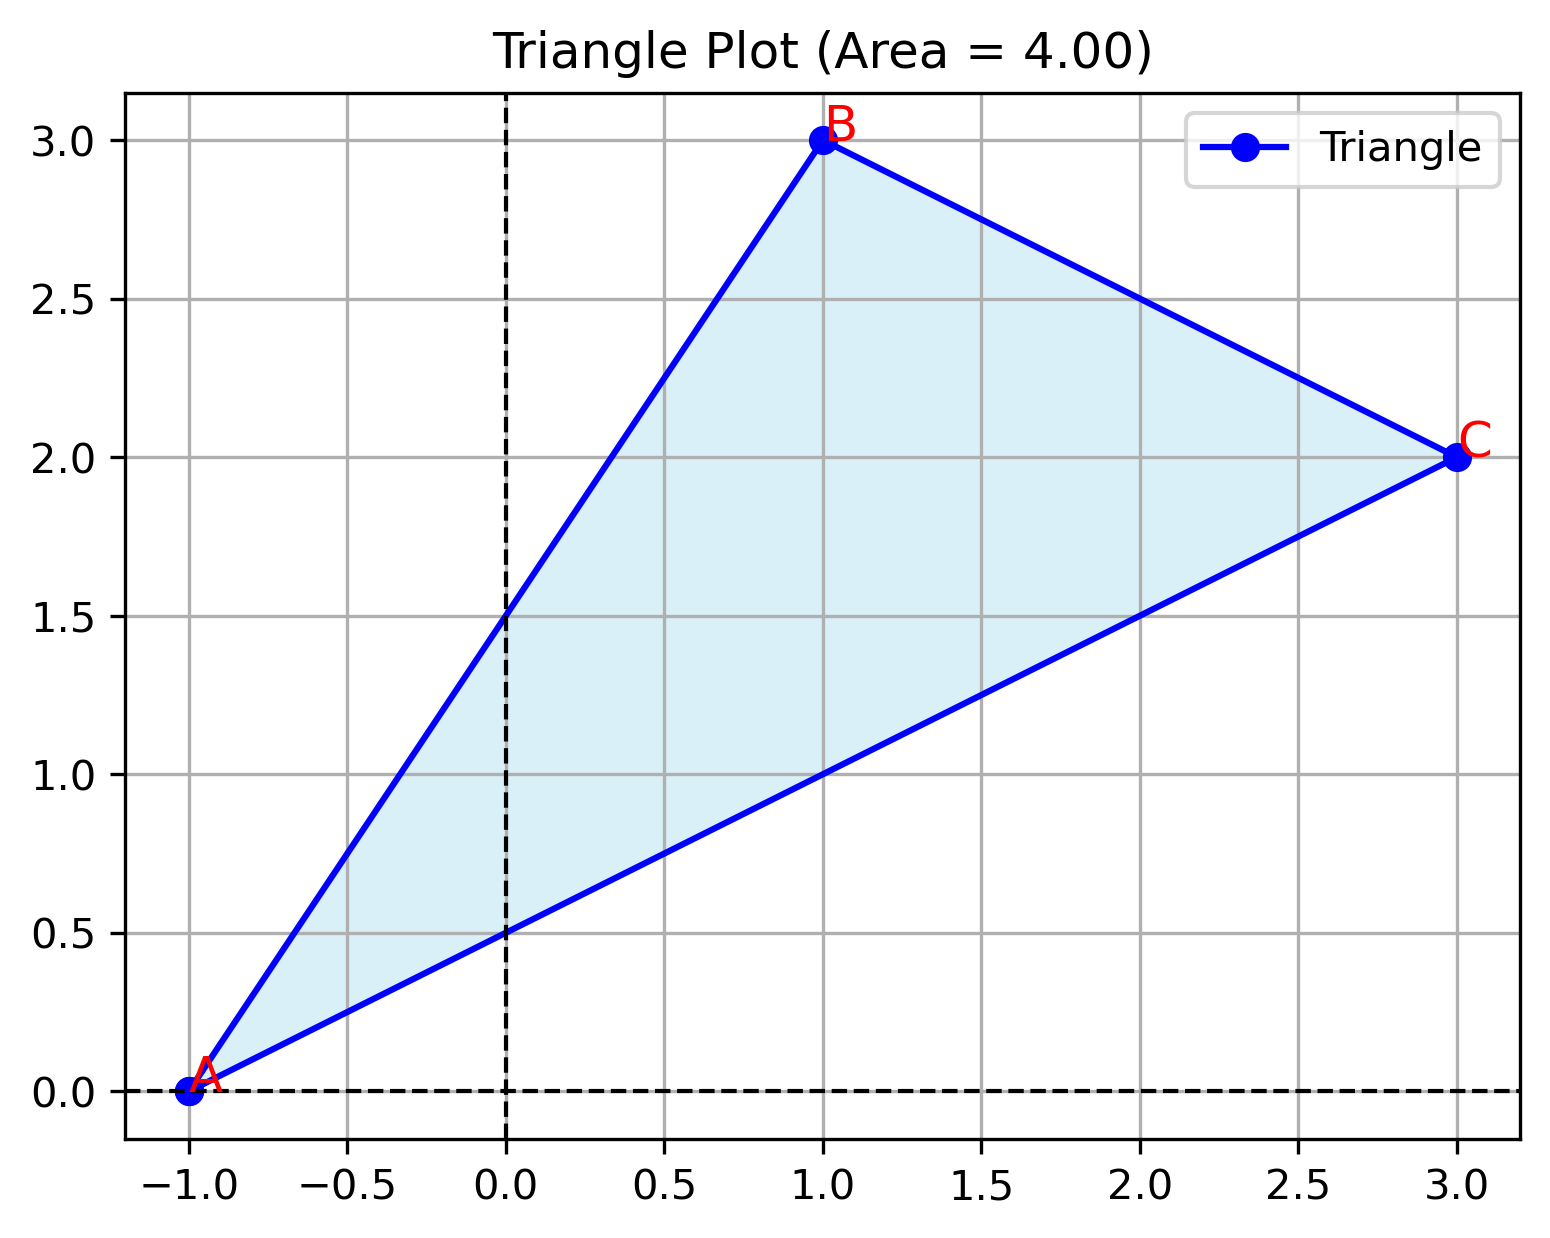
\includegraphics[width=\columnwidth, height=0.8\textheight, keepaspectratio]{../figs/triangle_plot.png}     
\end{frame}


\begin{frame}[fragile]                            
\frametitle{C code - To calculate the area of triangle and Save points}                
\begin{lstlisting}
#include <stdio.h>
#include <stdlib.h>
#include <math.h>
#include "/home/dhanush-kumar-a/ee1030-2025/ai25btech11010/matgeo/1.11.12/codes/libs/matfun.h"

int main() {
    // Step 1: Create triangle vertices as 2x1 matrices
    double **A = createMat(2,1);
    double **B = createMat(2,1);
    double **C = createMat(2,1);

    A[0][0] = -1; A[1][0] = 0;
    B[0][0] = 1;  B[1][0] = 3;
    C[0][0] = 3;  C[1][0] = 2;
    \end{lstlisting}

\end{frame}


\begin{frame}[fragile]                            
\frametitle{C code - To calculate the area of triangle and Save points}                
\begin{lstlisting}

    // Step 2: Compute vectors AB and AC using matrix subtraction
    double **AB = Matsub(B, A, 2, 1);
    double **AC = Matsub(C, A, 2, 1);

    // Step 3: Create rotated row vector [AB_y, -AB_x] for cross product
    double **rotAB = createMat(1,2);
    rotAB[0][0] = AB[1][0];   // AB_y
    rotAB[0][1] = -AB[0][0];  // -AB_x

    // Step 4: Area = 0.5 * |rotAB * AC|
    double **prod = Matmul(rotAB, AC, 1, 2, 1); // 1x1 matrix
    double area = 0.5 * fabs(prod[0][0]);
    \end{lstlisting}

\end{frame}


\begin{frame}[fragile]                            
\frametitle{C code - To calculate the area of triangle and Save points}                
\begin{lstlisting}

    // Step 5: Save results to files
    FILE *fp_points = fopen("points.dat", "w");
    if(fp_points != NULL){
        fprintf(fp_points, "Vertex\tX\tY\n");
        fprintf(fp_points, "A\t%.2f\t%.2f\n", A[0][0], A[1][0]);
        fprintf(fp_points, "B\t%.2f\t%.2f\n", B[0][0], B[1][0]);
        fprintf(fp_points, "C\t%.2f\t%.2f\n", C[0][0], C[1][0]);
        fclose(fp_points);
    }

    FILE *fp_area = fopen("area.dat", "w");
    if(fp_area != NULL){
        fprintf(fp_area, "%.2f\n", area);
        fclose(fp_area);
    }
    \end{lstlisting}

\end{frame}


\begin{frame}[fragile]                            
\frametitle{C code - To calculate the area of triangle and Save points}                
\begin{lstlisting}

    // Step 6: Free memory
    for(int i=0;i<2;i++){
        free(A[i]); free(B[i]); free(C[i]);
        free(AB[i]); free(AC[i]);
    }
    free(A); free(B); free(C);
    free(AB); free(AC);
    free(rotAB[0]); free(rotAB);
    free(prod[0]); free(prod);

    return 0;
}

\end{lstlisting}
\end{frame}

	
\begin{frame}[fragile]                              
	\frametitle{Python code -Ploting the points using c function}
		\begin{lstlisting}

import os
import numpy as np
import matplotlib.pyplot as plt

# Step 1: Compile the C program
os.system("gcc c.c -o triangle -lm")

# Step 2: Run the compiled C program
os.system("./triangle")

# Step 3: Load points data
points_data = np.genfromtxt("points.dat", skip_header=1, dtype=None, encoding="utf-8")
labels = [row[0] for row in points_data]
x_vals = np.array([float(row[1]) for row in points_data])
y_vals = np.array([float(row[2]) for row in points_data])
\end{lstlisting}
\end{frame}

	
\begin{frame}[fragile]                              
	\frametitle{Python code -Ploting the points using c function}
		\begin{lstlisting}

# Step 4: Load area
with open("area.dat") as f:
    area = float(f.read().strip())

# Step 5: Prepare triangle coordinates
triangle_coords = [(x_vals[i], y_vals[i]) for i in range(3)]
triangle_coords.append(triangle_coords[0])  # close the triangle
tx, ty = zip(*triangle_coords)

# Step 6: Plot the triangle
fig, ax = plt.subplots(figsize=(6,6))
ax.plot(tx, ty, 'b-o', label='Triangle')
ax.fill(tx, ty, 'skyblue', alpha=0.3)
\end{lstlisting}
\end{frame}

	
\begin{frame}[fragile]                              
	\frametitle{Python code -Ploting the points using c function}
		\begin{lstlisting}

# Label points
for i in range(3):
    ax.text(x_vals[i], y_vals[i], f"{labels[i]}", fontsize=12, color='red')

# Axes formatting
ax.axhline(0, color="black", linewidth=1.0, linestyle="--")
ax.axvline(0, color="black", linewidth=1.0, linestyle="--")
ax.set_aspect("equal")
ax.grid(True)
ax.set_title(f"Triangle Plot (Area = {area:.2f})")
plt.legend()
\end{lstlisting}
\end{frame}

	
\begin{frame}[fragile]                              
	\frametitle{Python code -Ploting the points using c function}
		\begin{lstlisting}

# Step 7: Save and show plot
os.makedirs("../figs", exist_ok=True)
plt.savefig("../figs/triangle_plot.png", dpi=300, bbox_inches="tight")
plt.show()
	
\end{lstlisting}                               
\end{frame}

\begin{frame}{Plot-Using  Python and C}
    \centering
    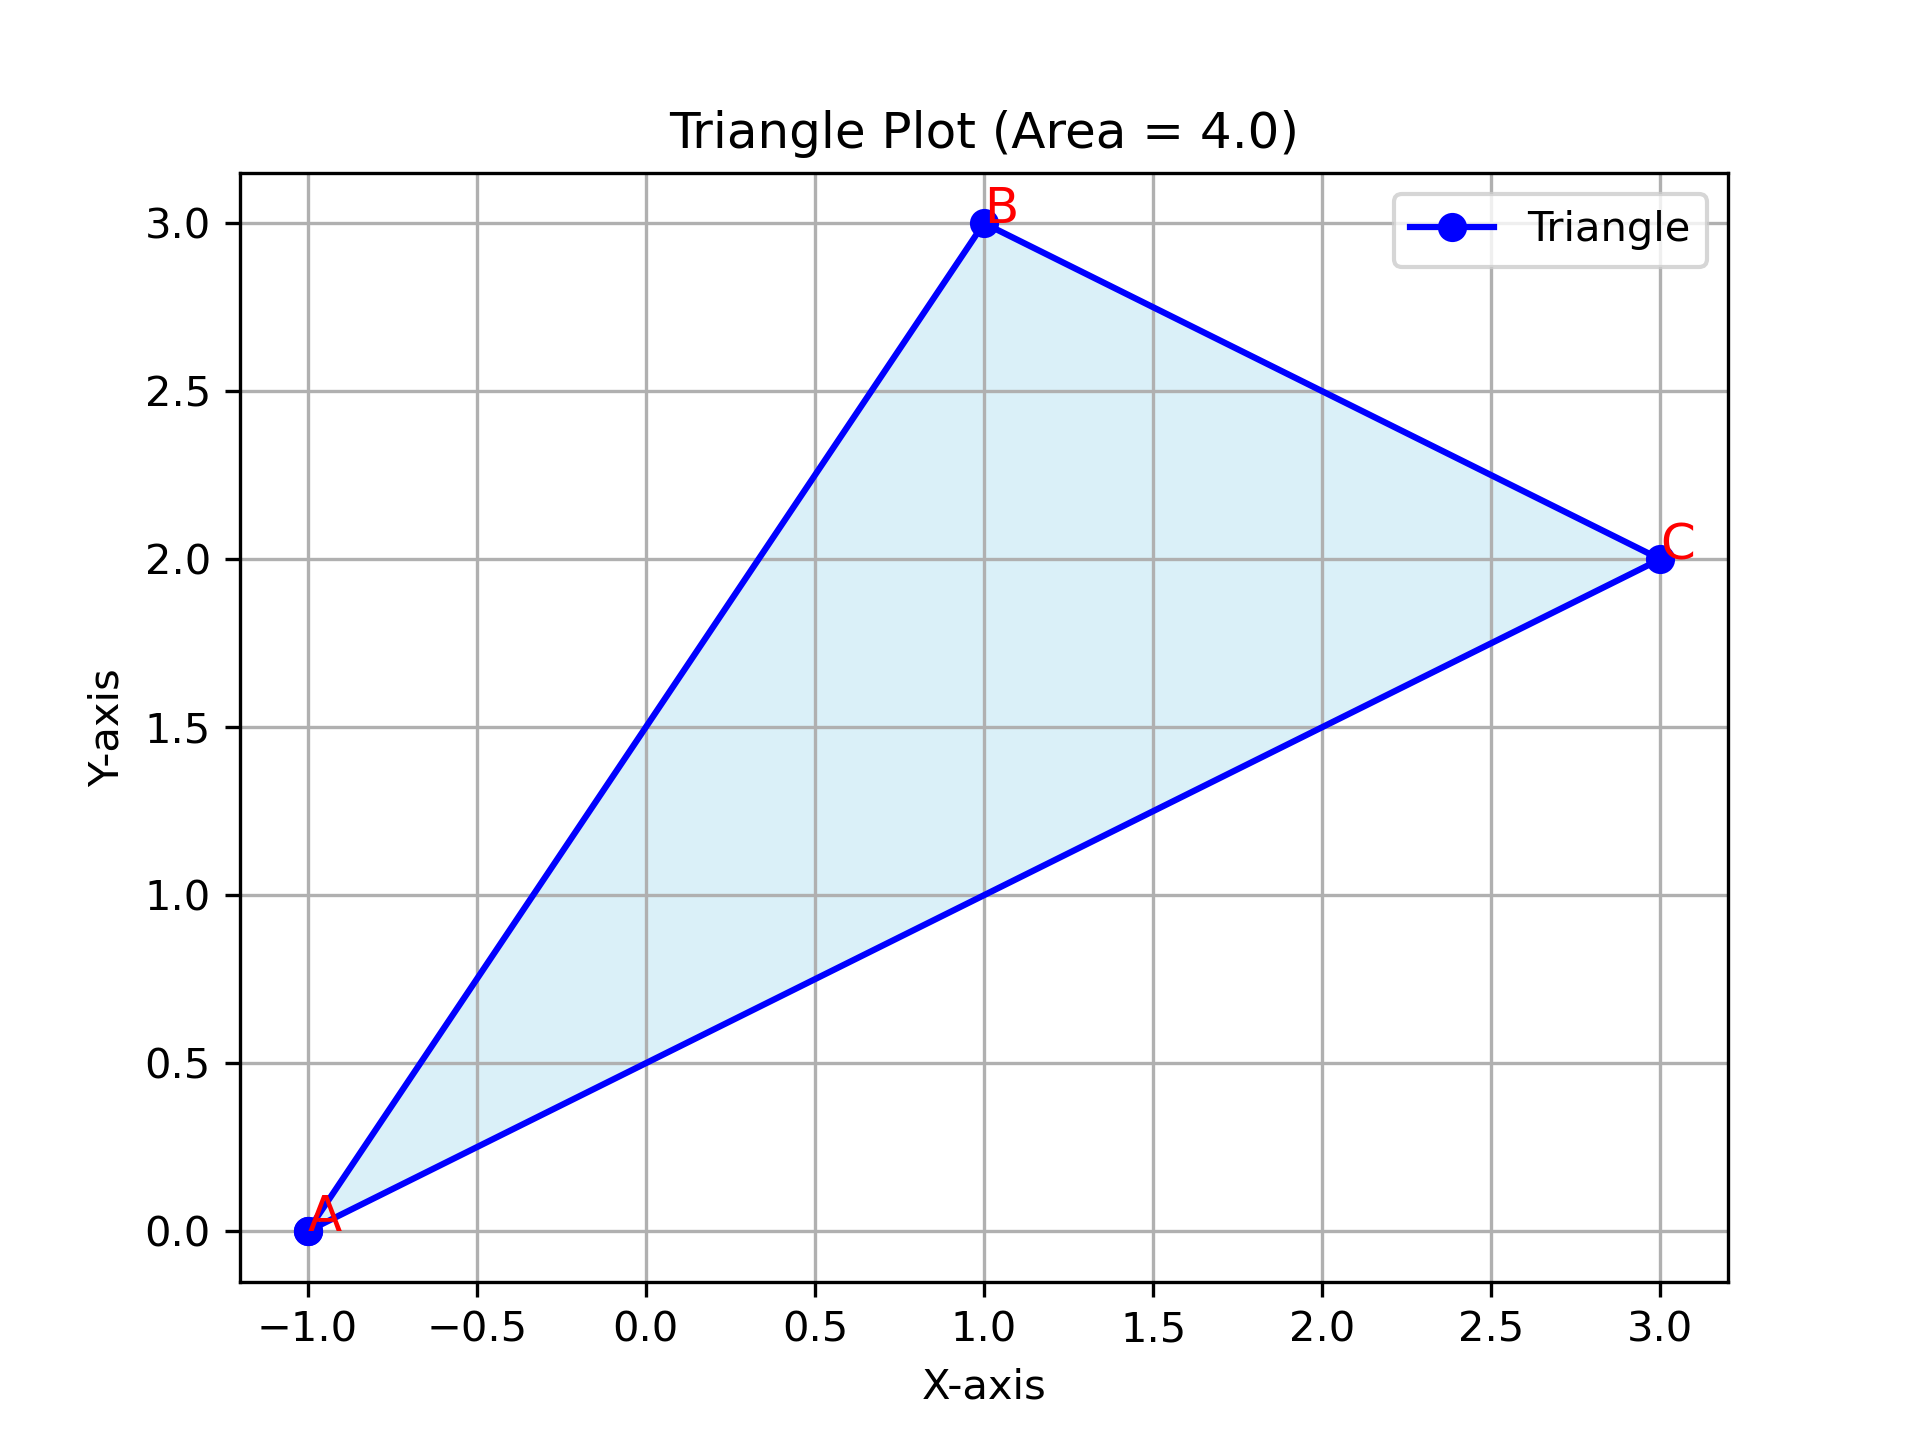
\includegraphics[width=\columnwidth, height=0.8\textheight, keepaspectratio]{../figs/triangle_plot1.png}     
\end{frame}

	


\end{document}
